\chapter{Improvements}
\label{chapter:improvements}

\section{Automation}

Using the study plug-in a mixing engineer will not have to draw gain automations manually. Nevertheless it can be useful to have an automation drawn by the plug-in. On one hand side it visualises the adapted gain curve better than the gain slider contained in the UI alone. On the other hand, it can save up calculation resources when the plug-in reads its own automation instead of processing the same vocal track in a repeated way. This is not necessary in simple mixing sessions but comes in handy when the mixed musical piece contains a great number of tracks with even more digital effects on each channel. Every digital effect increases the total amount of necessary CPU power. Often single tracks are bounced in place\footnote{all effects are rendered and combined with the actual signal to a new audio file} to avoid problems in performance. When the plug-in just reads an automation it is no considerable part of this problem even if there are multiple vocal tracks using this effect.\\
For those reasons the study plug-in was extended with this feature. In principle automations are supported by the JUCE framework and it can be very simple to implement a standard automation process. The normal case would be a user interacting with the UI and the plug-in communicating these changes to the DAW on write mode. On automation read mode the changes are send back to the plug-in during playback and it does its normal processing chain with changing parameters with the user drawn timing. The study plug-in was a special case which made it more difficult to realise the automation. In case of the study plug-in the write process of the automation should not be influenced by a user at intended use. Furthermore it should just receive and multiply the adapted gain from the drawn automation at read mode.\\
Like in the Waves plug-in a button was implemented at the UI to switch between read and write mode. Therefore the plug-in always knows if it needs to adapt the gain itself. The read mode implementation was performed quite fast as it just bypasses the regular calculations and multiplies the gain value set by the DAW with the current sample. The communication between DAW and plug-in works well on this part with the predefined parameter class from JUCE. The write mode produced more problems.\\
The plug-in adapts the gain value at write mode for every sample. When this would be communicated to the DAW like in normal automation process it has to draw at least 44100 adapted gain values each second. This easily overtaxes a DAW and is more accurate as it needs to be for a acceptable result. The DAW expects just a few changes per second for the automation as its normal use case (user modifies parameter at UI) would generate. It follows that the drawn automation had to be simplified.\\
At the first attempts automation changes were only communicated when the gain adaption changes its direction (compression/amplification) or when the difference to the last drawn automation point became crucial. Unfortunately this did not work as well. The output in the DAW would have been acceptable but at some spots it made incorrect jumps. These jumps occured in duration of at most 2 samples but they were still unwanted. Due to involvement of several devices in this process the real cause of the jumps could not be figured out. Different timings and positions for the communication to the DAW and also change of the parameter values were tested. During an long early testing phase no difference or worse results were achieved before an acceptable result was found:\\
The final solution sets a automation point every 80ms as long the gain changed about at least 0.1dB.
Therefore the gain adaption is constantly drawn in the automation curve but 12,5 instead of 41000 times a second or more. It does not set a new point when the gain is not adapting as this would be redundant. There are still jumps in the curve but this is acceptable as the jumps occur rarely and gain difference is about at most 0.1dB. Additionally these jumps are now located at correct positions without smoothing, which is not essential for such small amounts of adaption.\\

\begin{figure}[H]
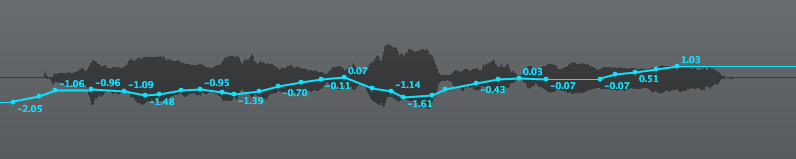
\includegraphics[width=\textwidth]{images/automation}
\caption{Automation written by the study plug-in into a DAW}
\end{figure}

\section{Adapting Loudness Goal}

The loudnessGoal parameter is not regarded as a gain controller. It is not designed to amplify the signal to a desired level. Instead, it should be adjusted to the actual loudness of the signal. In this way the plug-in can use its full range for changes on dynamics. For example when the loudnessGoal is set far below the signal level, the plug-in will stay at its minimal allowed gain value (initalized with -6dB) as long as it gets the high-level input. Even if it is at one end of the user defined dynamic range it will still operate in half (only negative/positive gain adaption) for most of the time. Therefore it is important to set the loudnessGoal correctly. In best practice the plug-in will compress the incoming signal as much as amplifying it.\\
To simplify the selection of a fitting loudnessGoal for a user, a input meter was implemented close to the loudnessGoal slider and the current gain adaption. In this way it is easier to check whether the current setting makes sense. However it still remains a problem as the perfect loudness goal possibly alters through a song. As a consequence it is difficult for a human to guess the average setting for the entire musical piece. Therefore some calculation-based solutions were tested.\\
The first approach was determining a new loudnessGoal for every second. To achieve this the plug-in summed up all resulting gain values for each sample in this time period. Afterwards it calculated the average tendency (more positive or more negative gain values). The offset was finally subtracted from the current loudnessGoal and the sum of the gain values got reset.\\
Problematic with this approach was that the loudnessGoal adaption was one second too late if the signal level changed. In addition it diminished some advantages of the plug-in as it treated different parts of the vocals with different settings which results in some local benefits but leads to varying level through the whole track.\\
As a consequence analysing parts of the vocal track only would not lead to a profitable result. Furthermore, the plug-in should go through all critical parts of its input and therefore decide for the best suiting loudnessGoal. In conclusion a button was implemented accessible at the UI which switches the plug-in to loudnessGoal detection mode. During the time this mode is active the plug-in will not multiply the calculated gain with the signal but is still determining it, dissimilar to a regular bypass. In addition the plug-in re-adjusts its allowed gainRange for this period of time to the maximum (+/- 10dB). This is done to find a most accurate average loudness rate and it has no negative consequences as it endures as long as the detection mode is active. If the plug-in is run in detection mode through the full vocal track it calculates a decent loudnessGoal. To avoid the result being falsified by sections without vocal signal, it only adapts on input with actual signal.\\
This is a task predestined to be performed offline, but due to the complexity of offline calculations in a plug-in operating in different DAWs the resources to realise it were not available in this study. For future work it would be possible to make use of the full ITU-R BS.1770-4 algorithm for this task.\\
Although the loudnessGoal detection mode is probably the best current way to set the parameter, it is still allowed for a user to choose it manually for own creative reasons.\\
When the loudnessGoal algorithmically adapts or is set to a new value chosen by the user the threshold of the plug-ins gate will change as well. Regardless of whether the average input is of low or high level the plug-in is thus able to handle it with reasonable settings.\\

\section{Side Chain}

So far the plug-in works well on single audio tracks and reduces long term dynamics. This substantially lessens the work for a mixing engineer but a average vocal level staying constant during a whole musical piece is not necessary the wanted result. If the instrumental backtracks varies in loudness it is desirable for the plug-in to vary its output gain accordingly. To realise this variation the plug-in requires additional information. Therefore a side chain input was added to the plug-in's interface.\\
Side chaining is not part of the standard I/O\footnote{I/O = input/output} layout of JUCE but is supported since JUCE version 4.1. To realise another input, it was added in the BusesProperties() structure from the AudioProcessor class. As for the plug-in it is not necessary to have a side chain input, supported bus layouts had not to be changed. Therefore the embedding DAW is able to feed it with a signal but does not need to do so. For further testing in Logic Pro 9 the plug-in had to be revalidated for the DAW, before it accepted the new I/O layout. This was not necessary for previous algorithmic changes.\\
After implementing the new input the new information had to be processed. To do this the plug-in reads the side chain buffer in its main processBlock() method. Information about the loudness of the backtrack (which should be fed into the side chain) is needed to enable determination of a useful additional output gain. In process of detecting the loudness of the side chain input it is passing through the filter, RMS and gain calculations like the regular input signal (see Fig. 5.2). Passing includes transformation into logarithmic number space. Afterwards it is compared to the current loudnessGoal and the calculated difference is smoothed. Now the smoothed gain is transferred back to linear number space and it is multiplied with the gain of the parallel determination from the main input.\\
It is important for the side chain processing not to interfere with the main input gain calculations of the plug-in. Especially the loudnessGoal must not be changed through this process. Otherwise it would corrupt its results in terms of dynamic range and make the loudnessGoal detection useless.\\
While testing in real use cases it was found beneficial to add an additional output gain for the finally returned signal. This reduced the effort of matching vocal output level with the backtrack. It would be an advantage if the plug-in could set the output gain itself depending on the side chain input, but as for different music styles and creative decisions there is not one correct version of vocal to backtrack relation but a great number of reasonable options could be appropriate. Nevertheless during future improvements of the plug-in this part could be simplified in its user interaction.\\
The side chain feature remains an usable addition to the main plug-in but becomes no part of it as it is not automatically profitable in every use case. That is why a button is implemented at the UI to toggle side chain integration on and off. On further term this is useful as different DAWs will handle an undefined (when no input channel/bus is chosen) side chain input in a dissimilar. For example will Logic Pro 9 send an empty signal containing only zero values. This would effect the outcome of the plug-in when side chain integration is active as it would interpret the signal as a quiet backtrack. With the side chain activation button toggled off by default, there is no urgent need of a silence detection always running in the plug-ins side chain processing chain.\\
A remaining question for the side chain implementation related to setting of the average time coefficients for RMS calculations and gain adaption (see 5.6). On one hand it should not react on small changes (for example when a musician is just accentuating certain beats in the backtrack), on the other hand it needs to react fast enough to calculate an appropriate gain for the first words of a new song part with a different loudness level. It is not negligible that it operates with the lookahead already realised for the plug-ins main use.\\
Additionally, in the first approach it turned out to be a difficult problem for the side chain gain adaption to deal with instrumental breaks of longer duration (up to a full bar). While most of the instruments are pausing during those breaks the vocals should stay at the same level as it is often used to emphasize the remaining musicians. With the current implementation of side chain adaption instrumental breaks were causing a parallel slowly falling vocal level. After the implementation of the idle time (see below) at gain adaption this behaviour could be avoided for the most part.\\

\begin{figure}[H]
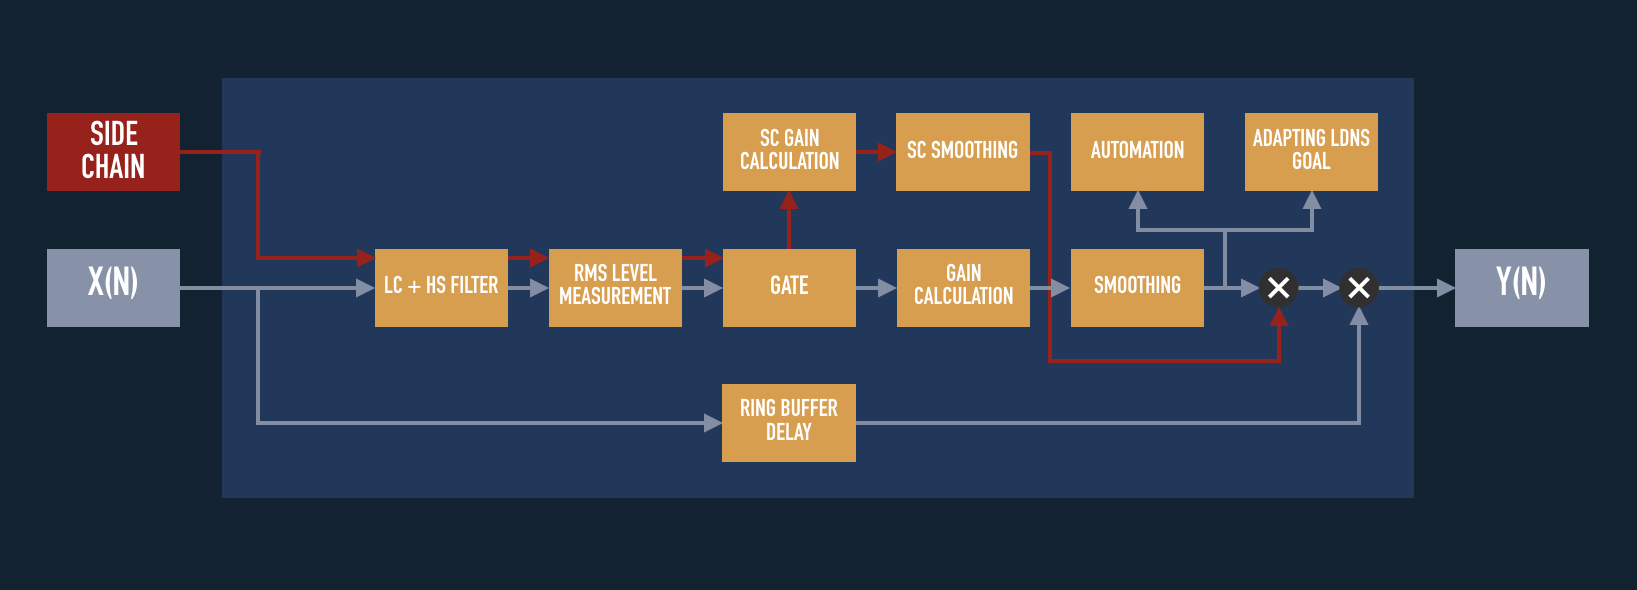
\includegraphics[width=\textwidth]{images/chain02}
\caption{Improved processing chain}
\end{figure}

\section{Idle Time}

During the comparison of the study plug-in with the “Vocal Rider” the idea of implementing a idle time before fading to 0dB gain emerged. The effect an idle time is that the plug-in will ignore short gaps between vocal signals. Therefore the plug-in does not change the adapted gain for example when a singer does a short rhythmic break in his/her vocals. So it will just use the actual vocals in the input for gain adaption similar to how a mixing engineer would do it. Due to a reasonable short duration of the idle time it is still able to adapt to 0dB gain for parts without singing. Subsequently there will be no risk of amplifying unwanted noise. The short period after a vocal signal and before a part of silence were the plug-in is still idle will not remain much longer than the vocal decay and is even shortened by the amount of lookahead delay.\\
At the first approach in implementing this feature the function of the gate was expanded. Each time the input dropped below threshold, the current sample was replaced by the last one above threshold during the set amount of idle time. Due to the fact that the last sample above threshold is still being at comparably low level it did not work as expected. The subsequent gain adapting was consequently falling on even lower results than without the change at the gate because at idle time it got values near the lowest possible one which was just not set to the loudnessGoal by the gate. It is assumed that the error could be fixed by replacing the samples at idle time with a RMS value from a sample further ahead, but this would require a additional memory space for past samples and it seemed to be too complicated for this study.\\
Therefore, the current implementation is based on the plan that the plug-in should detect at the gate whether there is no vocal signal and then freeze the current gain at the following gain adaption. As the gain adaption is much slower due to compress/amplification time smoothing than the RMS averaging before the gate, it freezes the gain before it is able to adapt to the level change. For reasons of simplification everything was implemented in the updateGain method.\\

\begin{lstlisting}[frame=single]
double AutoVocalCtrlAudioProcessor::updateGain(double sample, 
double lastGn)
{
    if (sample != *loudnessGoal) {
        idleCount = 0;
    } else if (idleCount < maxIdleSamples) {
        idleCount++;
        return lastGn;
    }
...
}
\end{lstlisting}

This algorithm detects whether the current level is below gate threshold by comparing the sample with the loudnessGoal. If the transferred RMS averaged sample is at the exact value of the loudnessGoal it can be assumed that the gate replaced its actual value. The rare case of a sample being randomly at exact the level of the loudnessGoal and therefore stop the gain adaption cant be eliminated in this implementation. Nevertheless, this makes no noticeable difference as it just stops the slow gain adaption for one single sample (max 1/44100 sec in expected use case). At the first sample differing from the loudnessGoal the idle timer is reset and the gain adaption continuous. When the maximum idle time is reached it has the same effect apart from resetting the idle time counter.\\
With the idle time working well in the main processing chain of the plug-in, its advantages in terms of side chain integration were evaluated. With the plug-in version developed so far there was still a problem related to instrumental breaks and their unwanted impact on the calculated gain correction. Therefore a implementation of idle time similar to the already existing one for the main input was used. At the final side chain calculations it was implemented and adjusted the length of the maximum idle time with tests in a real mixing environment. The result with a reasonable set maximum was quite acceptable as it substantially reduced the gain drop during instrumental breaks as long as the side chain input level was adapted to the loudnessGoal. Consequently the UI was expanded with a pre-gain slider for the side chain input which adds up before the comparison to the loudnessGoal. Controlling the input level of the side chain signal was possible before via a level-controlled bus\footnote{A Bus is a single path for multiple audio sources to be routed and processed.} send but now the mixing engineer is able to do it all at one place while check the level meters for both signals right next to each other at the UI. As it was still difficult to adjust it correctly for a whole song a self setting algorithm for the input gain was added to the already existing detection mode. As said before this would be significantly better realised in an offline thread but also works in real time for now.\\

\begin{figure}[H]
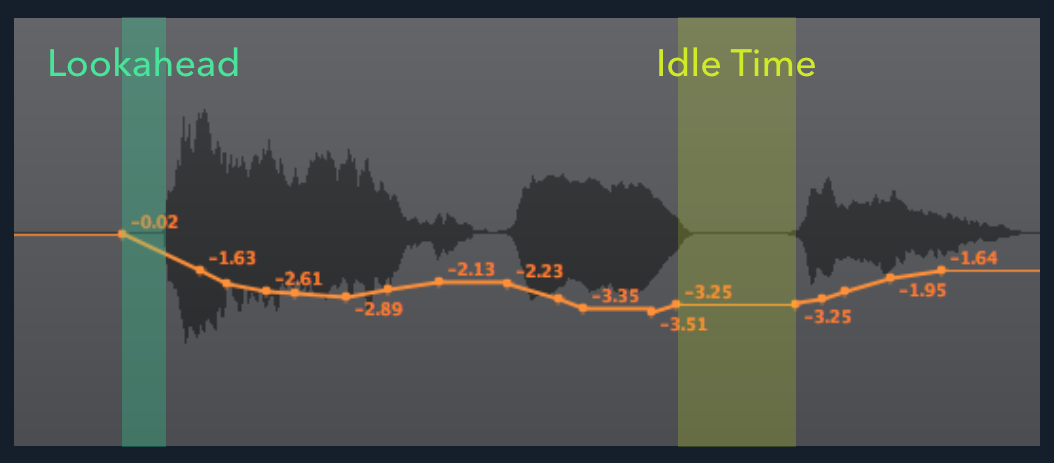
\includegraphics[width=0.8\textwidth]{images/automation2LookIdle}
	\centering
	\caption{Idle time and lookahead marked at automation written by the study plug-in}
\end{figure}

\section{Wet/Dry}

Many plug-in effects for DAWs have an additional slider to adjust the wet/dry ratio of their outcome. In these terms 100% “dry” is similar to the signal without the effect and 100% “wet” is a fully processed effect on the signal. This reduces the effort which would be necessary for sending the signal on a second track with the effect inserted to mix both tracks together in wanted proportions.\\
In consideration of the use of such a slider in the plug-in of this thesis, it seemed useful at first as it ables a user to set the intensity of dynamic compression. On the other hand this is already possible in a slightly different way with better outcome, by changing the current gainRange. In addition that this is feature has its main use in creative work, which is not the main objective of this plug-in, the final plug-in will not include a wet/dry slider for now. This decision was made with the intension of simplifying the UI to its foundation followed by the reduction of the settable parameters.\\

\section{Parameter Reduction}

As the plug-in slowly reaches its final state, it was necessary to transfer some settable parameters to fixed constants. In development it was useful to be able to change the important parameters while in runtime for example the compress and amplification times. Now it already emphasised which settings will  result in the best outcome. Small changes could be slightly better depending on the current circumstances but they are not required for a good result. Additionally with wrong application these parameters could create a poor result. Therefore and with the likely possibilities of a user not knowing what each of these parameters does, it seemed to be advantageous to hide those as constants, invisible at the UI.\\
This parameter reduction was applied to the lookahead delay, compress time, amplification time, RMS time, idle time, the side chain time constants and like already described, the gate. With the experience from testing the plug-in with many different settings in various circumstances the default choices for the parameters already got to reasonable values.\\
With a bad lookahead delay the gain adaption could happen to early or it has no noticeable effect. In the process of testing it commuted in at 60ms of delay as a good default value. For the parameter reduction it got set to 50ms as this resulted in the best outcome at additional test with special precision on the lookahead delay. A further test with a comparison of the drawn automation and the vocal signal waveform validated the new setting (see Fig. 5.1, 5.3).\\
The RMS averaging time shouldn’t be to long as this adds up on the total reaction time of the plug-in. On the other hand it needs a big enough time window to calculate a useful average. At the beginning of development it was set to 60ms. The comparison to the Waves “Vocal Rider” resulted in very small time windows (down to 8ms) for the averaging at this plug-in, to imitate the outcome. As this seemed a bit fast in consideration of previous experiences, it got into further tests with altering RMS time in collaboration with changing compress and amplification times. As result the RMS time is finally set to 30ms.\\
With the initialisation of two different attack times for compression and expansion it was manifested that the expansion time would be greater then the compression time. Still the final settings were not yet set. So again, the comparison to the “Vocal Rider” served as an inspiration. Though with a expansion time above two seconds it was not reacting fast enough to achieve the planned results, especially compared to the compression. As consequence the expansion time came down to 1500ms for the final build.\\
The compression time results from the comparison with the “Vocal Rider” were similar to a slow compressor and therefore still to fast to fit the idea of this thesis. As follows it had to be tested independently. This lastly resulted in a compression time of 600ms working out and, even though it was not planned, a slope of 1/3 at gain reduction. The reason for a additional slope were some vocal parts which got their level to low after compression. With a slope only at compression the gain adaption is balanced.\\
The idle time is set after considerations on the small gaps between phrases on vocal tracks. As it should be long enough to endure most of these gaps it is finally set to 500ms. A longer duration for the main functionality of the plug-in seemed unreasonable as it mainly extends the part after a vocal signal where the plug-in would just amplify noise.\\
For the side chain input the plug-in takes a idle time set to two seconds to be able to ignore instrumental breaks. With a shorter setting it still results in decreasing vocal level while those breaks are happening. Furthermore it uses the same RMS time like the main input and smoothes the resulting gain similar slow to the amplification time with a time coefficient adjusted to 1600ms.\\
The gate just adapts with the loudnessGoal like described in 5.2 and is not settable in the UI anymore.\\

\section{Final Gain Clipping}

Due to the problems of a possible disproportional gain (see 3.6) caused by an unexpected error, it needs to be checked before it is finally multiplied with the plug-in’s input signal. This includes the gain of the plug-ins main functionality the additional side chain gain and the user set output gain. It is not easy to set a good clip range as with 3 different gain values multiplied it can result in high amplification which can still be wanted. In todays DAWs usually clipping at 1.0 in linear number space is only happening at the master fader. As consequence it is unproblematic to mix a single audio track above this threshold as long as the final mix will happen below. Therefore it is not reasonable to clip the gain*input product for +/- 1.0 sample values.\\
As consequence not the final outcome could be clipped but the final multiplied gain which includes all three gain variables. The clip was set to operate in the linear number space as last instance before the final multiplication. It clips the final gain for the range of 0.0 to 6.0. The clipping range starts at 0.0 because negative gain in the linear number space does not make sense in this context as it would only invert the phase of the input signal in addition to the compression or amplification. 6.0 is the clip in terms of amplification which is similar to a approximately 15dB gain boost. This is lower than the highest value that can be achieved with all gain sliders on maximum setting but this is not expected to happen in reasonable use. With a clip at 6.0 the input signal is already able to be amplified by 600\%. If a signal needs stronger amplification in professional mixing it is presumable that the setting was done wrong or the recording is bad and should be replaced. If this could not be done or is not wanted it is necessary to edit the audio track before the start of the mixing session as the plug-in is not able to handle it alone. Since this case is still unlikely to occur in professional mixing the plug-in stays within the safety clipping range that will fit its intended use cases.\\

\section{Store Settings}

At startup the plug-in regularly initialises with settings that may fit some use cases but always have to be checked and adjusted properly for the current audio tracks. As a mixing engineer could start a mixing process on one day and finish it on another he may save and close the project and the used DAW for the night. Therefore the plug-in needs to get its latest settings saved or else it would initialise with the unchanged startup setting. This problem already effects the UI at runtime when it is closed and opened again. While the parameters for processing still stay correct in this case the UI could show wrong values at sliders which are not correctly refreshed.\\
To prevent this problem the getStateInformation() and setStateInformation() which will be called by the DAWs are filled with the necessary save commands.\\

\begin{lstlisting}[frame=single]
void AutoVocalCtrlAudioProcessor::setStateInformation (const 
void* data, int sizeInBytes)
{
    ScopedPointer<XmlElement> xmlState (getXmlFromBinary (data, 
    sizeInBytes));
    if (xmlState != nullptr)
    {
        if (xmlState->hasTagName ("AutoVocalCtrl"))
        {
            *sc = (bool) xmlState
            ->getBoolAttribute ("sc", false);
            *read = (bool) xmlState
            ->getBoolAttribute ("read", false);
           ...
            *loudnessGoal = (float) xmlState
            ->getDoubleAttribute ("loudnessGoal", -20.0);
            *gainRange = (float) xmlState
            ->getDoubleAttribute ("gainRange", 6.0);
            ...
        }
    }
    ...
}
\end{lstlisting}

The plug-in creates a new xml file with the values of all settable parameters in the getStateInformation() method and reads the xml file for parameter adjustment in the setStateInformation() method. Finally the setStateInformation() method notices the UI to refresh the according parameter sliders.\\
As DAWs are calling those methods at different timing but always at startup and before the shutdown of the plug-in or the UI, all user made adjustments are saved and regained at startup. Additional in this way the DAW will be able save presets for the plug-in which can be used in other mixing session for example as orientation for the parameter adjustment.\\

\section{UI Design}

The main focus of this study was the algorithm behind the plug-in. Nevertheless it was the intension that a user should be able to work with the plug-in without reading a manual. Therefore the UI was refactored after parameter reduction.\\
The main problem of the previous UI was the lack of the possibility to differ between sliders for parameter adjustments and elements which were displaying inside information of the plug-in (see Fig. 5.4). Additionally the slider labels had not enough space to display in complete length similar to the slider value displays which could already confuse a user by their large number.\\

\begin{figure}[H]
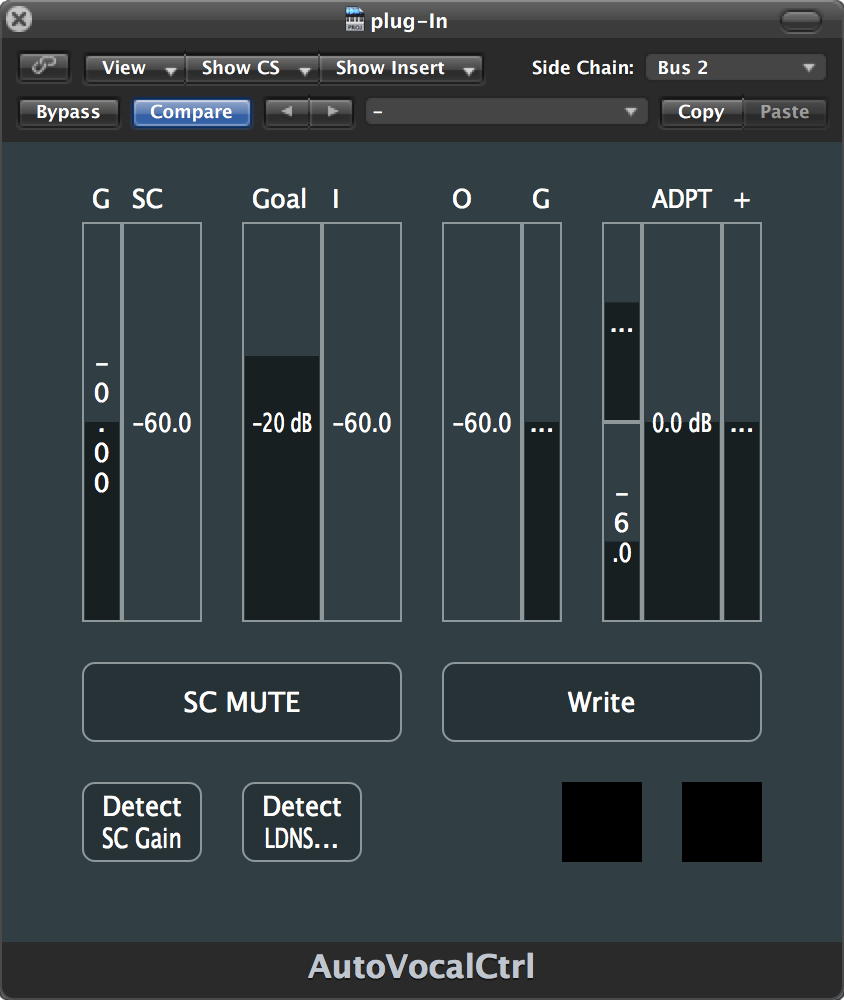
\includegraphics[width=0.5\textwidth]{images/designVorher}
	\centering
	\caption{UI after parameter reduction}
\end{figure}

The main change in the UI re-design was the highlighting of usable elements. To set them apart from only informational parts, all the changeable components are coloured red. The colour is chosen as it strongly diverges from its complementary colour green which is the plug-in’s main colour (see Fig. 5.5). Additionally only the usable sliders and buttons got a coloured frame instead of the plain black outline of the pure metering components.\\

\begin{figure}[H]
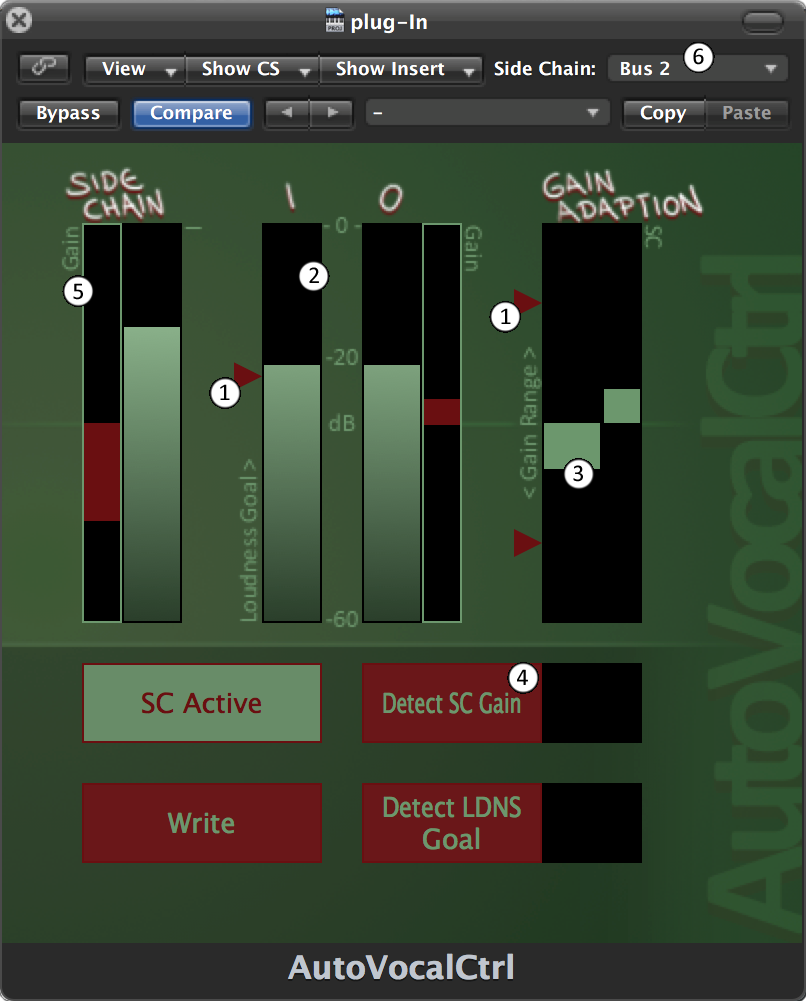
\includegraphics[width=0.5\textwidth]{images/designNeuNum}
	\centering
	\caption{Final UI in Logic Pro 9}
\end{figure}

In the new design the gain range and loudness goal are set via red triangles (1) pointing on the corresponding level/gain meter. This was done to let the user to know the connection between these UI elements. The loudnessGoal should be set in consideration of the input level meter (2) right next to it and the gain range is directly modifying the maximal and minimal values of the connected gain reduction meter (3).\\
The three meters which are displaying the I/O levels (input, side chain input, output) are next to each other and visualising their value with a rising bar where a colour gradient is applied to. Therefore the green tone of the bar is getting brighter with increasing signal level to support a fast assessment of the user.\\
All UI elements excluding the buttons are divided in different sections: The I (input), O (output), side chain and gain adaption section, containing the belonging components. To know which task the single components fulfil, they have a additional label, on the side which is not adjoining to another UI element.\\
When the Side Chain feature is disabled, the corresponding gain detection button (4) and the side chain input gain slider (5) become disabled too, as they would have no effect. This can be observed by the user as the red colour of these UI elements gets greyer and the slider loses its green frame which previously signalled a possible interaction. The components which are only for displaying information are disabled for user interaction by default.\\
For most of the slider elements it is not necessary for the user to know the exact value but to get a approximation and therefore a feeling about what is happening. Clear slider values often seduce users to adjust sliders to pretty numbers (e.g. rounding to 5 or repeated digits) instead of only observing the change of the outcome. As consequence most of the slider values are removed in the new design. A orientation for the input and output meters is still located next to them but in a light green like the element labels in order to not distract from the main information.\\
The side chain input (6) is chosen in the embedding DAW and therefore not to set in the plug-in’s UI.\\